\section{Wstęp}

Polskie góry od zawsze cieszyły się niezwykłą popularnością wśród turystów zarówno z kraju, jak i z zagranicy. Nie jest to nic dziwnego, polskie szczyty są dosyć niskie i możliwe do zdobycia dla większości ludzi, gdyż nie wymagają ani profesjonalnego sprzętu, ani kondycji fizycznej wieloletniego sportowca.
W erze mobilności i posiadania wszystkiego na wyciągnięcie ręki coraz mniej zwiedzających decyduje się na korzystanie z tradycyjnych map papierowych z wyznaczonymi szlakami górskimi. Mapy papierowe oczywiście są bardzo dobrym, sprawdzonym rozwiązaniem, lecz są podatne na zniszczenie przez zamoczenie czy podarcie. Ponadto zajmują miejsce w plecaku turysty i często sprawiają problem z ich poprawnym złożeniem, zwłaszcza będąc na szlaku. Posługiwanie się nimi wymaga także przynajmniej podstawowej umiejętności odczytywania danych z mapy oraz dobrej orientacji w terenie i obsługi kompasu. Mapy mobilne niwelują wiele z tych problemów, a przy okazji ułatwiają poruszanie się po szlakach, ponieważ wykorzystując moduł GPS w urządzeniu mobilnym, pokazują na bieżąco położenie wędrowca.

Już w 2. połowie XIX wieku turystyka górska zyskała znaczną popularność, w szczególności w Tatrach. Niezbadane i nieoznakowane dotąd tereny budziły zainteresowanie podróżników, którzy wyrażali chęć powołania stowarzyszenia łączącego pasjonatów wypraw górskich. Dlatego już w 1873 roku powstało Towarzystwo Tatrzańskie, pierwsza taka organizacja na ziemiach polskich i szósta na świecie \cite{ptt}. Członkom Towarzystwa zależało przede wszystkim na zbadaniu Karpat, ochronie przyrody, w szczególności zwierząt alpejskich oraz rozpowszechnianiu zebranych informacji o tym paśmie górskim celem jeszcze większego spopularyzowania turystyki górskiej na terenie Polski i ułatwieniu zainteresowanym zwiedzania, a także wsparciu szeroko pojętego przemysłu górskiego. Za poboczny cel utworzenia Towarzystwa można również uznać chęć zjednoczenia narodu polskiego, żyjącego w tamtych latach pod zaborami, jako próba wspólnego wystąpienia przeciwko wrogom. Towarzystwo w 1920 roku zmieniło swoją nazwę na Polskie Towarzystwo Tatrzańskie, lecz jego cele pozostały bez zmian. Dzięki jego działalności rejony Tatr cieszyły się tak wielkim zainteresowaniem, że już w 1889 roku zauważono potrzebę podjęcia odpowiednich kroków w celu ochrony przyrody, jednak Tatrzański Park Narodowy utworzony został dopiero po wojnie w 1954 roku \cite{tpn}.

Fakt, iż polskie Tatry cieszą się ogromną popularnością potwierdzają poniższe wykresy stworzone na podstawie statystyk prowadzonych przez Tatrzański Park Narodowy \cite{tpnstat}. Turyści najchętniej wędrują po Tatrach w lecie, gdy warunki atmosferyczne pozwalają na korzystanie z wyznaczonych szlaków bez konieczności zaopatrzenia się w profesjonalny sprzęt wspinaczkowy, lecz zimą to pasmo górskie także cieszy się popularnością podróżników \ref{sprzedaz2023}. Wykres \ref{sprzedaz} pokazuje stale rosnące zainteresowanie turystyką górską w tym regionie. 

\begin{figure}[H]
    \centering
    \fbox{\includegraphics[scale=1]{img/wykresy/sprzedaż 2023.jpg}}
    \caption{Wykres przedstawiający liczbę sprzedanych biletów wstępu na teren Tatrzańskiego Parku Narodowego w poszczególnych miesiącach 2023 roku.
}
    \label{sprzedaz2023}
\end{figure}

\begin{figure}[H]
    \centering
    \fbox{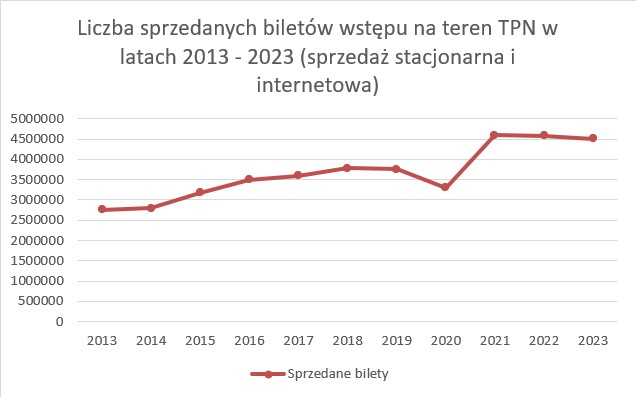
\includegraphics[scale=1]{img/wykresy/sprzedaż ogółem.jpg}}
    \caption{Wykres przedstawiający liczbę biletów wstępu na teren Tatrzańskiego Parku Narodowego w latach 2013 - 2023 sprzedanych łącznie stacjonarnie i internetowo.}
    \label{sprzedaz}
\end{figure}
 
Niniejsza praca opisuje rozwiązanie problemu nawigowania po szlakach górskich w polskiej części Tatr. Harnasie to aplikacja mobilna, która ułatwia poruszanie się po górach, z gwarancją bezpieczeństwa podczas wędrówki. Aplikacja oprócz nawigowania po szlakach posiada funkcję zgłaszania zagrożenia występującego na danym szlaku. Użytkownik może powiadomić innych turystów o niebezpieczeństwie, jak również otrzymać informację o zagrożeniu na trasie, na której aktualnie się znajduje. Baza danych wykorzystywana w aplikacji zawiera informacje o użytkownikach korzystających z tej aplikacji, szlakach oraz powiadomieniach opisujących zagrożenie na trasie. Potrzeba stworzenia takiej aplikacji jest duża. Harnasie dają gwarancję bezpieczeństwa oraz pewność, iż każdy, kto będzie z niej korzystał, nie zabłądzi i zostanie powiadomiony o wszystkich występujących zagrożeniach.

W kolejnych rozdziałach opisane zostały najważniejsze elementy mające wpływ na jakość tworzonej aplikacji. Praca zawiera również opis użytych technologii oraz wszystkich funkcji, które posiada aplikacja. Dzięki temu czytelnik może zapoznać się z budową aplikacji oraz zasadami jej działania. Niektóre funkcje aplikacji zostały zaprogramowane na podstawie znajomości działania popularnych aplikacji, obsługujących śledzenie trasy przy wykorzystaniu modułu GPS. Wiedza ta znacznie ułatwiła rozwiązanie pewnych problemów dotyczących wyznaczania trasy oraz modyfikowania jej, gdy system znajdzie lepszą drogę.

Zwieńczenie pracy stanowi rozdział \ref{wnioski}. Prezentuje on wnioski końcowe na temat stworzonej aplikacji.

\newpage
